\subsection{\LARGE Exploring the Hardware Limitations}

Before showing project results and benefits of parallel execution, we will take a look on limits we encountered. 

\subsubsection{\textbf{\large CPU limitations}}

\begin{itemize}
    \item The process of sequentially learning and simulating physics on a CPU has been found to be quite slow, particularly when dealing with a relatively high number of instances. Specifically, it has been observed that at around 300 instances, a single iteration \footnote{In this paper, iterations and frames are used interchangeably and each frame corresponds to a single learning and simulation step along with a visual output. Paper also mentions a real-time learning, which here corresponds to approximately 25 frames per second. Although 25 frames per second may not be ideal for interactive applications, it is worth noting that movies are typically shot at 24 frames per second and still appear smooth to viewers. However, we will still aim to present the examples at about 60 frames per second.} of the simulation takes approximately one second to complete. Given that an episode typically lasts between 200 and 400 iterations, this would mean that it would take approximately one hour to complete 10 generations of the simulation. This presents a significant challenge in terms of computational efficiency and highlights the need for more powerful and efficient hardware to effectively handle larger datasets and more complex simulations and that is where the GPU comes.
\end{itemize}

\subsubsection{\textbf{\large GPU limitations}}

\begin{itemize}
    \item The \textbf{visualization} component of the algorithm was able to sustain the rendering of approximately 4 million instances at a rate of 60 iterations per second. The primary requirement for this step was the PosVelBuffer, which consumed a total memory of 1.2-1.5GB on the GPU. The ShapeShader, which is responsible for generating additional 3D coordinates for each connection, further expanded this memory requirement to 4.5-5.0GB. Despite the GPU having a total memory of 6GB, the inclusion of other data such as textures for display resulted in a near-limit usage of memory, which ultimately resulted in a drastic decrease in performance if we were to increase the instance count any further.

    \item The integration of the \textbf{simulation} component with visualization resulted in a noticeable decrease in performance compared to visualization alone. The algorithm was only able to sustain the rendering of approximately 1 million instances at a rate of 60 iterations per second. Despite the inclusion of additional buffers, none were able to match the memory requirement of the PosVelBuffer. Though the reduction in the number of instances resulted in a decrease in memory usage by about 75\%, the addition of physics algorithms and dense computations significantly slowed down the overall performance of the algorithm.

    \item The integration of the \textbf{learning} component with simulation and visualization proved to be the most challenging aspect of the algorithm testing. Each instance required its own neural network, represented by a 3-layered structure. The total matrix size for this component was staggering, with 6000 floats per instance. This represented a significant increase in memory requirements, with a 2 orders of magnitude increase from the previous memory requirements for visualization and simulation alone. This resulted in a return of the previous memory bottleneck, compounded by the intense nature of matrix multiplication and the simultaneous access of a large number of threads to the main memory. As a result, the algorithm was only able to sustain the rendering of 50,000 instances at the end of the testing with 60 iteration per second.

    \begin{figure}[hbt!]
        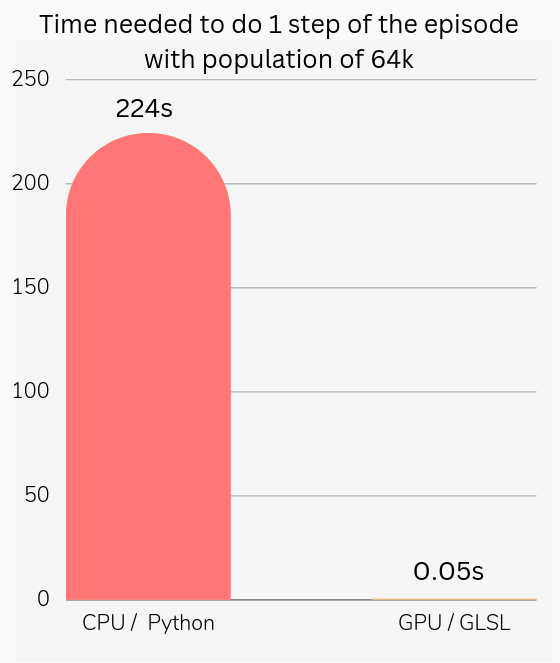
\includegraphics[width=3in]{time1step.png} %veličina u odnosu na širinu linije
        \caption{Illustration of advantage of using GPU's to simulate physics and run creature learning.}
        \label{fig:struktura} %label mora biti drugaciji za svaku sliku
    \end{figure}

    \begin{figure}[hbt!]
        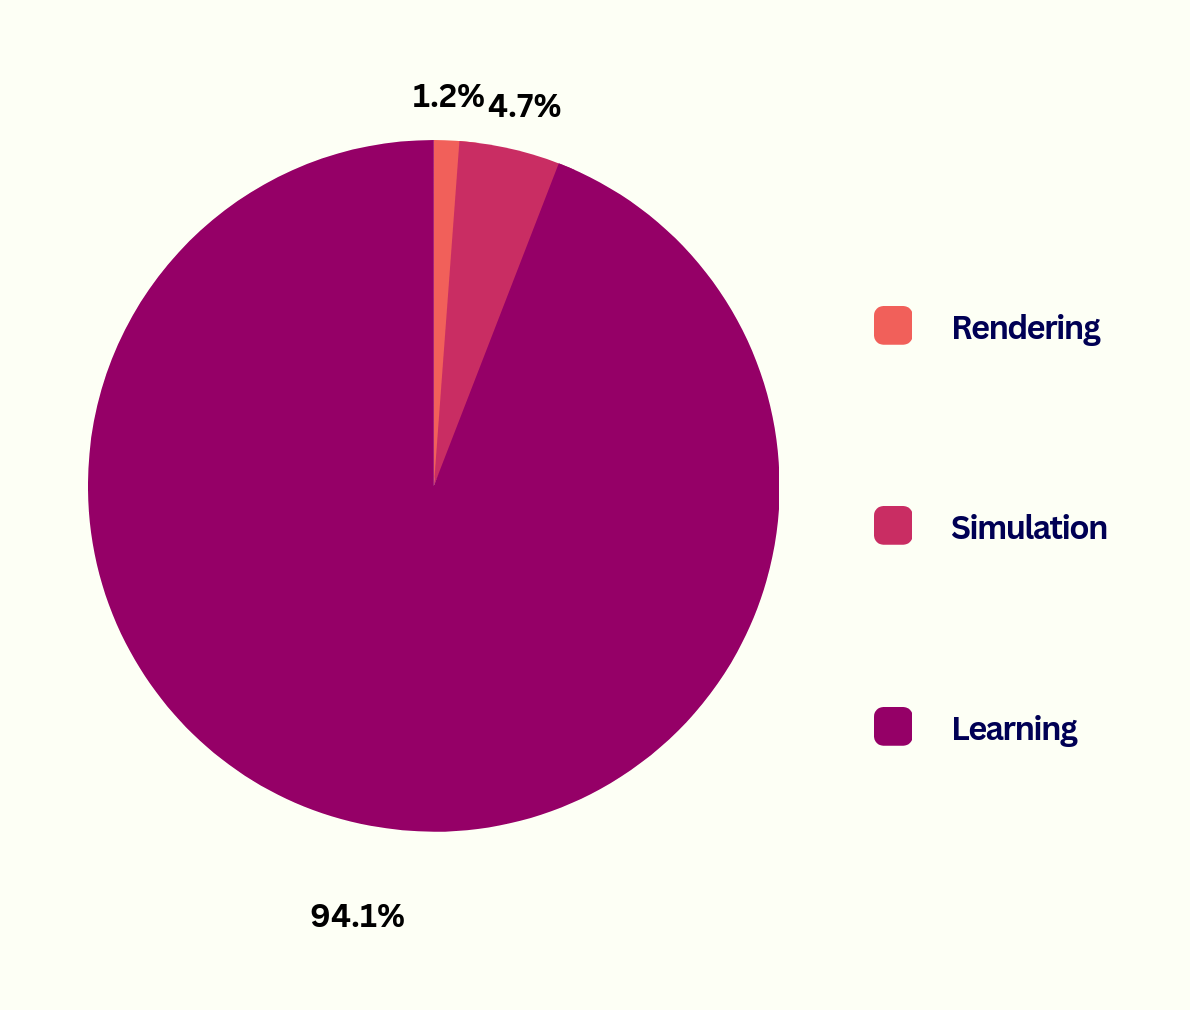
\includegraphics[width=3in]{resources/amdalh.png} %veličina u odnosu na širinu linije
        \caption{An illustration of Amdahl's law in practice. While we could have focused on improving the rendering or simulation the bulk of the time was spent on multiplying matrices, so we decided to leave rendering and simulation and focus on improving learning.}
        \label{fig:struktura} %label mora biti drugaciji za svaku sliku
    \end{figure}
        
\end{itemize}

% \clearpage

\subsection{\LARGE Unveiling the Results}


The next few figures showcase the different performances we get when we employ the CPU or the GPU for our task. \\


Figure 3. illustrates the efficiency of using a GPU to run simulations and evolution, as the GPU time per episode step is much less than the CPU time for larger population sizes. This highlights the advantage of using specialized hardware like a GPU for these types of computationally intensive tasks. \\


Figure 4. showcases the relationship between population size and the number of generations needed for creatures to learn to walk. As the population size increases, the probability that any creature will learn to walk by chance rises. This result suggests that a larger population size can lead to faster convergence and better performance in evolutionary algorithms. \\


\begin{figure}[H]
    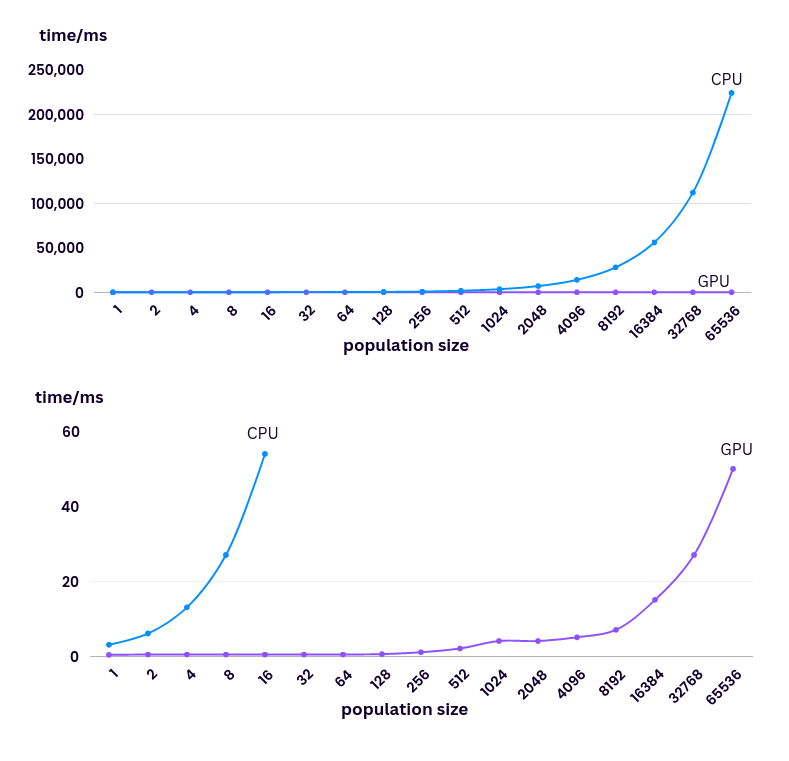
\includegraphics[width=3in]{popsizetime.png} %veličina u odnosu na širinu linije
    \caption{GPU vs CPU time per 1 episode step for different population sizes. GPU is running a program written in GLSL and CPU in Python. It can be seen that the CPU time grows much more quickly.}
    \label{fig:struktura} %label mora biti drugaciji za svaku sliku
\end{figure}

\begin{figure}[H]
    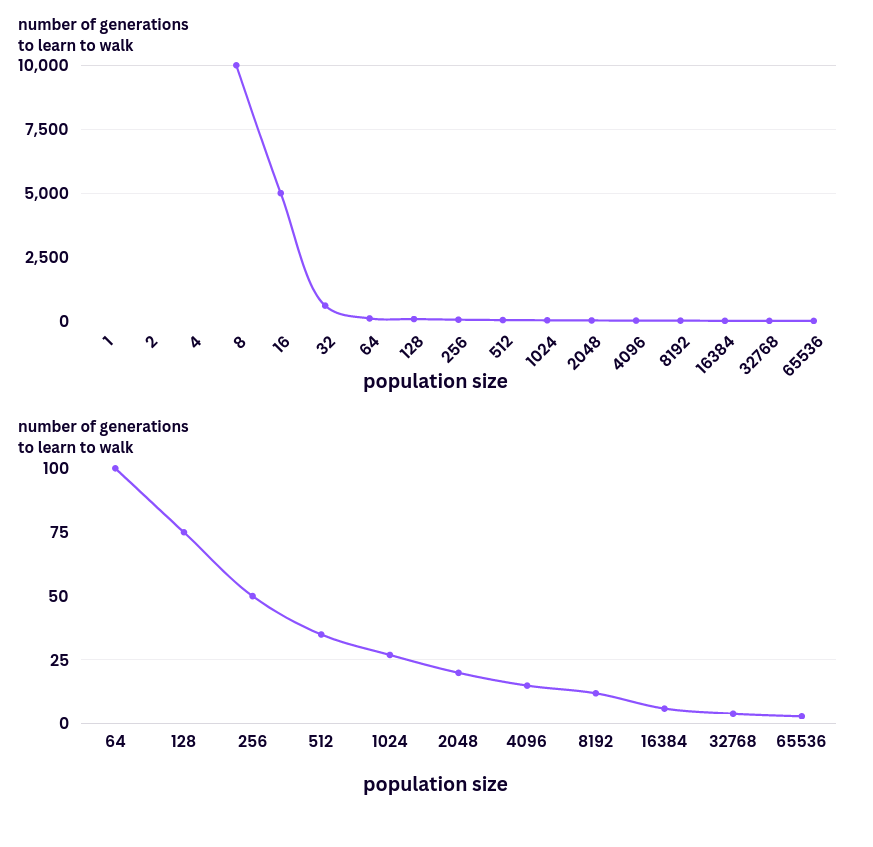
\includegraphics[width=3in]{numberofgenerationstolearntowalk.png} %veličina u odnosu na širinu linije
    \caption{As the population size grows number of generations to learn to walk falls. This is because when the population size is large, the probability that any creature is walking by pure chance is high.}
    \label{fig:struktura} %label mora biti drugaciji za svaku sliku
\end{figure}


